\section{Versuchsauswertung}

\subsection{Standard-Versuchsanlage} 

\subsubsection{Dimensionierung des MAGs}
Für die Inbetriebnahme der Standard-Druckanlage sollte zunächst die Dimensionierung des Ausdehnungsgefäßes (MAG) mit Hilfe der Gleichung nach Schnauss erfolgen.  Nach folgender Gleichung X gilt [aus Praktikumsskript entnommen]: 

\begin{equation}
\label{eq:eff.VolMAG}
V_u= \frac{(V_t * C_e + V_{vap} + V_r)*(p_{max} + 1)}{(p_{max}-p_{min})}
\end{equation}

\begin{center}
	\begin{small}
		$V_u$: Effektives Volumen des MAGs,
		$V_t$: Flüssigkeitsvolumen des Solarkreises,
		$C_e$: Ausdehnungskoeffizient des Wärmeträgerfluids,
		$V_{vap}$: entstehendes Dampfvolumen im Stagnationsfall,
		$V_r$: Reservevolumen,
		$p_{max}$:maximaler Druck $=p_vs*0,9$,
		$p_{min}$: minimaler Druck,
		$p_{vs}$: Auslösedruck des Sicherheitsventils.
	\end{small}
\end{center}

Das Flüssigkeitsvolumen des Solarkreises setzt sich aus den Volumen des Kollektors, dem Inhalt der Rohrleitung und dem Inhalts der Amaturen und des Wärmeübertragers zusammen. Bei dem Kollektor handelt es sich um einen Flachkollektor des Typ Vaillant auroTHERM classic VFK 140/2D* mit gutmütigem Ausdampfverhalten ohne direkten Verbindungsleitungen und einem Fluidinhalt von \SI{1,35}{\liter}. Für das Rohleitungssystem wurde eine Länge von \SI{30}{\metre} angenommen, bei denen es sich jeweils um \SI{50}{\percent} Kupferrohr des Typs DN15 (\SI{0,1771}{\litre\per\metre}) und \SI{50}{\percent} Edelstahl-WR DN16 (\SI{0,2641}{\litre\per\metre}). Der interne Wärmeübertrager wurde mit \SI{2}{\metre} Edelstahl-WR DN20 mit \SI{0,3941}{\litre\per\metre} angenommen. Die Anlagenhöhe beträgt ca. \SI{8}{\metre} und der Auslösedruck des Sicherheitsventils ist mit \SI{6}{\bar} angegeben. Als Wärmeträgerfluid wurde TYFOCOR LS angenommen. Aus dem Datenblatt wurde einen kubischer Ausdehnungskoeffizient für den maximalen Temperaturfall bei \SI{120}{\celsius} von \SI{74e-5}{\per\kelvin} Wärmefluids und eine Dichte von \SI{1013,5}{\kg\per\litre} für eine Umgebungstemperatur von \SI{25}{\celsius} approximiert. Unter der Angabe, dass der Kollektor keine direkte Verbindungsleitungen besitzt, beträgt das Verdampfungsvolumen näherungsweise dem Kollektorvolumen. Der minimale Anlagendruck beträgt dabei die Summe des statischen Drucks addiert zu \SI{0,5}{\bar} für den gasseitigen Druck und \SI{0,3}{\bar} für die Sicherheit. 

$V_u$ unter den angegebenen Bedingung folgenden Wert an:

\begin{equation*}
	\label{MAG-Ber.}
	\begin{aligned}
	V_u=  \SI{10,64}{\liter}
	\end{aligned}
\end{equation*}

\subsubsection{Anlagenleistung}

In der folgenden Abbildung sind die Einstrahlungwerte über den gesamten Messzeitraum von ca. \SI{54}{\minute} für die Standard-Versuchsanlage abgebildet. 
Die Einstrahlungswerte liegen über der durch die Norm spezifizierten Randbedingung von mind. \SI{800}{\watt\per\meter\squared} bei denen die Leistungsparameter bestimmt wurden. Für die Auswertung wurden die Daten im Scanbereich 874 bis 1088 verwendet.

\begin{figure}[H]
	\centering
	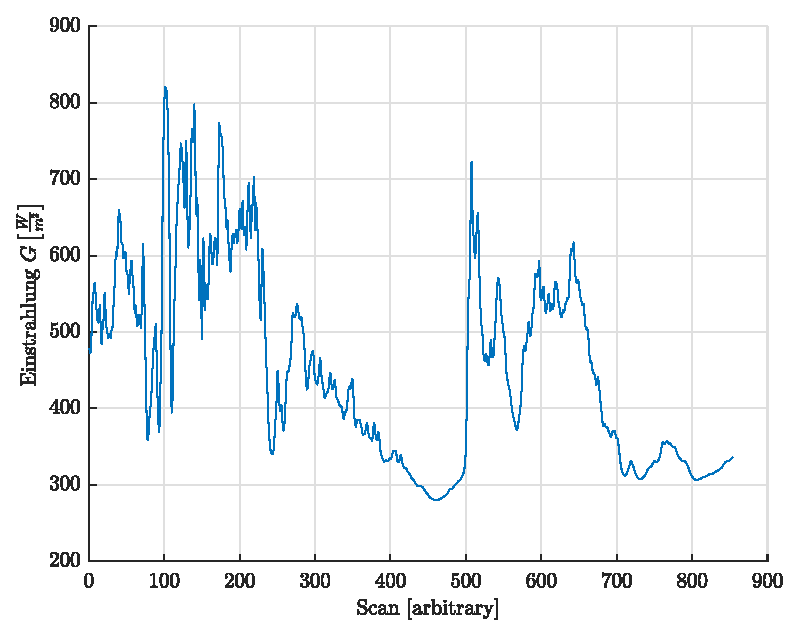
\includegraphics[height=0.3\textheight]{../DATA/DataEinstrahlung.eps}
	\caption[Gemessene Einstrahlung während der Betriebsdauer der Standard Versuchsanlage]{Gemessene Einstrahlung während der Betriebsdauer der Standard Versuchsanlage.}
	\label{fig:Einstrahlung}
\end{figure}

Für den definierten Messbereich ergibt sich eine Einstrahlleistung von \SI{1007.5(41)}{\watt\per\meter\squared}.

In der folgenden Abbildung wurde die momentane Kollektorleistung gegen den momentanen Anlagenwirkungsgrad dargestellt. 
Die momentane Kollektorleistung wurde nach Gleichung 2.4 des Praktikumsskripts berechnet. Der Anlagenwirkungsgrad wurden nach Gleichung 2.2 des Praktikumsskripts ermittelt. 

\begin{figure}[H]
	\centering
	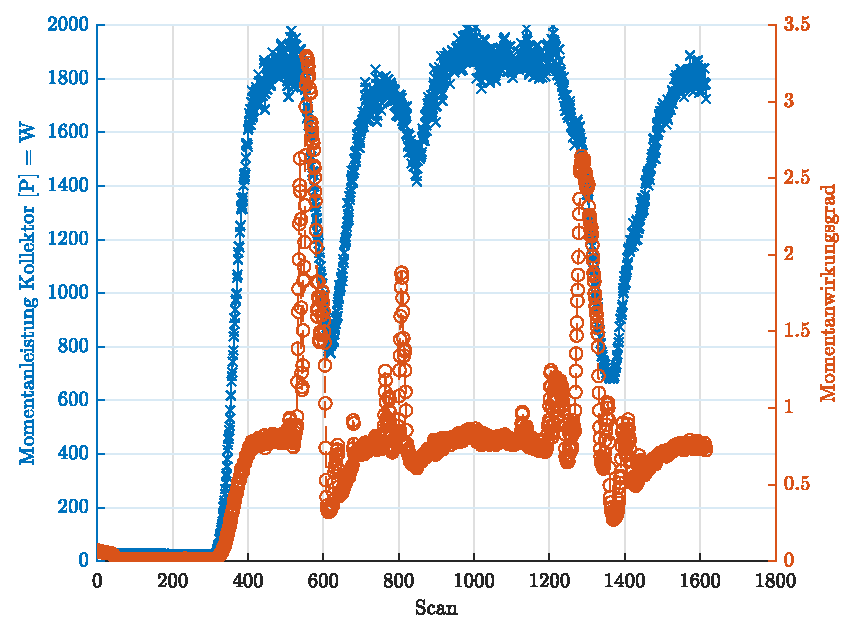
\includegraphics[height=0.3\textheight]{../DATA/LeistungTime.eps}
	\caption[Auftragung der Momentanleistung des Kollektors und des Momentanen Anlagenwirkungsgerades]{Auftragung der Momentanleistung des Kollektors und des Momentanen Anlagenwirkungsgerades.}
	\label{fig:Momentanleistung}
\end{figure}

Die theoretische Kennlinie des Kollektors wurde anhand der im Praktikumsskript angegebenen Daten für den Kollektor für Einstrahlungen von \SI{1000}{\watt\per\meter\squared}, \SI{800}{\watt\per\meter\squared} und \SI{600}{\watt\per\meter\squared} (schon unterhalb für die ermittelten Leistungsparameter benötigte Einstrahlung) berechnet und in der folgenden Abbildung dargestellt.

\begin{figure}[H]
	\centering
	\includegraphics[height=0.3\textheight]{../DATA/KennlinieTheo.eps}
	\caption[Theoretische Kennlinie des verwendeten Kollektors für Einstrahlwerte von von \SI{1000}{\watt\per\meter\squared}, \SI{800}{\watt\per\meter\squared} und \SI{600}{\watt\per\meter\squared}]{Theoretische Kennlinie des verwendeten Kollektors für Einstrahlwerte von von \SI{1000}{\watt\per\meter\squared}, \SI{800}{\watt\per\meter\squared} und \SI{600}{\watt\per\meter\squared}}
	\label{fig:KennKoll}
\end{figure}


\subsubsection{Fragestellungen}

\textbf{Funktioniert der in Betrieb genommene Kollektor wie erwartet?}

Dadurch, dass die Einstrahlungswerte am Tag des Versuchs durch relativ starke Bewölkung und immer wieder größerer Windentwicklung kam, kann anhand der Messdatenerfassung kein stationärer Betrieb angenommen werden. Die Einstrahlungswerte liegen grundsätzlich unter den vorgesehenen mind. \SI{800}{\watt\per\meter\squared}, da die Leistungsparameter der getesteten Kollektoren bei dieser Randbedingung bestimmt wurde. 

\textbf{Welche Messstellen braucht ein Solarregler mindestens für eine ordnungsgemäße
	Funktion? An welchen Positionen werden die Einschalttemperaturen für die Solarkreispumpe
	sinnvollerweise gemessen?}
Der Solarregler braucht Temperatursensoren für die Vor- und Rücklauftemperaturen am Kollektor und am Speicher. Die Temperatur sollte am Solarwärmeübertrager gemessen werden. 

\textbf{Wovon hängt die benötigte Pumpenleistung abhängig?}

Die benötigte Pumpenleistung hängt von der Länge des Rohrleitungssystems und der zu überwindenden Höhendifferenz vom Speicher zum Dach/der Kollektorfläche ab. 

\textbf{Warum wird die Solaranlage gespült?}

Die Solaranlage wird vor der Inbetriebnahme gespült, um die Luft aus dem Rohrleitungssystem und dem Kollektor zu drücken. Die Anlage muss über einen gewisschen Zeitraum gespült werden, damit auch Luft, die an Rohrknicken und Engstellen verweilt, aus der Apparatur abfließen kann.

\textbf{Warum darf keine Luft in der Anlage sein?}

Luft ist ein sehr schlechter Wärmeübertrager und mindert die Anlagenleistung des Solaranlage. In der Luft vorhandener Sauerstoff kann im Rohrsystem dazu führen, dass die Rohleitungen korrodieren. Große Luftmengen im System könne zusätzlich zu versagen der Pumpe führen. 

\textbf{Wozu ist ein Ausdehnungsgefäß vorzusehen und wonach richtet sich dessen Volumen?}

Veränderung der Umgebungstemperatur können zu Ausdehnung des Wärmetauscherfluids führen. Das Außgleichsgefäß führt mit seiner Membran dazu, dass der Systemdruck Im Stagnationsfall der Anlage fließt sämtliches Kollektorfluid in das Ausdehnungsgefäß, denn ein Verdampfen des Wärmefluids im Kollektor kann zum Auslösen des Überdruckventils und zur Zerstörung der Anlage führen. Im Stagnationsfall sollte daher das gesamte Kollektorvolumen in das Ausgleichsgefäß fließen können.

\subsection{Drainback-System}

\textbf{Vorteile eines Drainback-Systems gegenüber einem druckbehaftetetn System:}

Bei einer Drainback-Anlage wird kein externes Wärmeüberträgerfluid verwendet, sondern das Wasser aus dem Solarspeicher direkt durch den Kollektor gepumt wird. Beim Stillstand der Solaranlage läuft das gesamte Solarkreisvolumen in den Speichert zurück, sodass das Rohrsystem  komplett mit Luft gefüllt vorliegt. Es kann demzufolge nicht zu Frost- oder Überhitzungschäden oder Stagnation kommen, was den Einsatz gerade in sehr heißen klimatischen Gebieten ohne Stagnation ermöglicht. Der Instandhaltungsaufwand ist durch die Verwendung einer Drainback-Anlage geringer, da das System weniger thermischen Belastungen ausgesetzt ist und beispielsweise kein Ausdehnungsgefäß, Überdruckventile oder Frostschutzmittel benötigt. Dadurch gestaltet sich eine Drainback-Anlage häufig kostengünstiger, die Installation einfacher und die Lebensdauer in den meisten Fällen erhöht. \\

\textbf{Nachteile einer Drainback-Anlage:}

Damit der Kollektor einer Drainback-Solaranlage im Stillstandsfall leer fließen kann, muss der Kollektor der höchste Punkt der Anlage darstellen, zusätzlich muss zwischen dem Kollektor und der Solarstation ein Gefälle von mindestens \SI{4}{\percent} liegen, damit sich der Kollektor komplett entleeren kann. 
Der Abstand zwischen der Pumpe und dem höchsten Punkt des Kollektors sollte einen Höhenunterschied von ca. \SI{12}{\meter} nicht überschreiten, da eine Standard Hocheffizienz Umwälzpumpe eine größere Differenz nicht ohne stark erhöhte Kosten leisten kann und viel mehr Energie verbrauchen würde. \\

\textbf{Hydraulisches Phänomen beim Befüllen und Entleeren einer Drainback-Anlage:}

Um eine entleerte Drainback-Anlage zu befüllen muss eine bestimmte Pumpenleistung/Pumpendrehzahl verwendet werden. Durch Ausprobieren wurde eine Pumpenleistung von \SI{59}{\percent} ermittelt unter deren Bedingung sich der Solarkreis bis zum höchsten Punkt befüllte. Ist der Solarkreis mit Wasser gefüllt, kann die Pumpendrehzahl so weit zurück gedreht werden, dass bei Betrieb der Anlage nur noch \SI{5}{\percent} der Pumpenleistung benötigt werden. Dieses Phänomen kommt dadurch zustande, dass das in den Speicher herabfließende Wasser über ein statisches Vakuum frisches Wasser in den Solarkreis zieht. Aus diesen Gründen entleert sich bei Abstellen der Pumpe der gesamte Solarkreislauf. 

\subsection{Überprüfen des Wasser-Glykol-Gemischs}

Für den Versuch wurden drei Proben des Wärmeträgerfluid Wasser-Propylenglykol mit Hilfe eines Refraktometers untersucht. Das Refraktometer wurde mit destilliertem Wasser gereinigt und kalibriert. Anschließend wurden jeweils wenige Tropfen der Proben 1-3 auf die Probenträgerfläche gegeben und gegen das Licht gehalten. Über die Messskala konnten dann die Konzentration und der Gefrierpunkt der Mischung abgelesen werden. Es wurden folgende Beobachtungen gemacht:

\begin{table}[H]
	\caption{Mittels Refraktormeter ermittelte Glykolkonzentration und Gefrierpunkte der Wärmeübertragerfluidproben.}
	\centering
	\begin{tabular}{lcc}
		& Konzentration  & Gefrierpunkt \\
		&{[}\%{]}& {[}°C{]}\\
		Probe 1 &       44               &          -24           \\
		Probe 2 &       51            &            -32,5     \\
		Probe 3 &           30           &          -13             
	\end{tabular}
\end{table}

Probe 1 hatte ein klares orange/pink fluoreszierendes Aussehen. Die Glykolkonzentration liegt bei dieser Probe im gängigen Normbereich, es besteht kein Handlungsbedarf das Wärmeübertragefluid auszutauschen. 

Probe 2 zeigte eine etwas trübe bräunliche verschmutzte Färbung. Möglicherweise lag in der Solaranlage ein Stagnationsfall vor und das Wärmeträgerfluid wurde zu stark erhitzt. Die Konzentration und der Gefrierpunkt finden sich aber auch bei dieser Probe noch im Normbereich. 

Probe 3 lag tief braun und undurchsichtig vor.  Die Glykol-Konzentration im Wärmeübertragerfluid ist zu niedrig, sodass der Gefrierpunkt des Fluids mit \SI{-13}{\celsius} so gering ist, dass es zum Gefrieren des Fluid und in folge dessen zum Bersten der Apparatur kommen kann. Möglicherweise ist durch Überhitzen und einen/mehrere Stagnationsfälle Wärmeträgerfluid aus dem Solarkreis ausgetreten und es wurde dieser mit Wasser aufgefüllt. Möglicherweise ist das Wärmeträgerfluid durch zu starke Überhitzung zu schaden gekommen. Es sollte bei dieser Anlage unbedingt ausgetauscht werden und die Anlage vor erneuter Benutzung unbedingt gründlich gespült werden, um Verunreinigung und Schädigung weiterer Anlagenkomponenten zu vermeiden. 